\section{Spike-Train Decoding}
\label{sec:Spike-Train Decoding}

\begin{rem}
The decoding methods we have considered estimate or discriminate static
stimulus values on the basis of spike-count firing rates. Spike-count firing
rates do not provide sufficient information for reconstructing a stimulus
that varies during the course of a trial. Instead, we can estimate such a
stimulus from the sequence of firing times $t_{i}$ for $i=1,2,\cdots,n$ of the spikes
that it evokes. Here we can solve this problem in two ways, one is to allow time lag, and the firing sequence after time $t$ is also taken into account; the other is to introduce prediction, using the firing sequence before time $t$ to predict the stimulus at time $t$.
\end{rem}

\begin{asm}
  For simplicity, we restrict our discussion to the decoding of a single
neuron. We assume, as we did in chapter 2, that the time average of the
stimulus being estimated is $0$.
\end{asm}


\begin{prop}
  For the decoding of neurons, we may need to consider spikes for the
  following two time periods.
  \begin{enumerate}[(i)]
  \item   The firing of an action potential at time $t_{i}$ is only affected by
  the stimulus $s(t)$ prior to that time, $t<t_{i}$. That is, the
  evoked spikes tell us about the past behavior of the stimulus,and if stimulus have some
form of temporal correlation, that past behavior provides information
about the current stimulus value. Of course, if there is no correlation
between the stimulus $s$, then there is no need to consider the firing
sequence before time $t$.
\item The firing sequence after time $t$ is the neuron's encoding of the stimulus at time $t$ and the previous stimulus, so we must consider.
  \end{enumerate}

\end{prop}

\begin{prop}
  To make the decoding task easier, we
can introduce a prediction delay $\tau_{0}$, and attempt to construct, from spikes
occurring prior to time $t$, an estimate of the stimulus at time $t-\tau_{0}$. Such a delayed estimate uses a combination of spikes that
could have been fired in response to the stimulus $s(t-\tau_{0})$ being estimated
(those for which $t-\tau_{0}<t_i<t$), and spikes
(those for which $t_i<t-\tau_{0}$) which can contribute to its estimation on the basis
of stimulus correlations.

\end{prop}

\begin{rem}
  The estimation task gets easier
as $\tau_{0}$ is increased, but this delays the decoding and makes the result less
behaviorally relevant. We will consider decoding with an arbitrary delay
and later discuss how to set a specific value for $\tau_0$.
\end{rem}

\begin{prop}
  \label{prop:Spike-Train stimulus estimate}
  The stimulus estimate is constructed as a linear sum over all
  spikes. A spike occurring at time $t_{i}$ contributes a kernel
  $K(t-t_{i})$ , and the total estimate is obtained by summing over
  all spikes,
  \begin{equation}
    \label{eq:3.51}
    s_{\rm{est}(t-\tau_{0})}=\sum\limits_{i=1}^{n}K(t-t_i)-\left\langle r \right\rangle\int_{-\infty}^{\infty}K d\tau.
  \end{equation}
  The last term, with $\left\langle r \right\rangle=\left\langle n \right\rangle/T$ the average firing rate over the trial, is included to impose the condition that the time average $s_{\rm{est}}$ is $0$, in agreement with the time-average condition on $s$.
\end{prop}

\begin{defn}
  A kernel be imposed
by requiring $K(t-t_0)=0$ for $(t-t_i)\leq 0$ is termed causal.
\end{defn}

\begin{exm}
  \label{exm:3_13ABC}
  The sum in Equation \ref{eq:3.51}
  includes all spikes, according to Proposition \ref{prop:Spike-Train stimulus estimate} so only those spikes occurring prior to
the time $t$ (spikes $1-7$ in figure) should be included. The estimate is
obtained by summing the values of the kernels where they cross the dashed line
labeled $t$, for spikes up to and including spike $7$. The causal kernel is $0$
for negative values of its argument, so spikes for $i\geq 8$ do not
contribute to the estimate at this time. Figure A shows how spikes
contribute to a stimulus estimate,using the kernel shown in figure
B. For figure C, we will explain in the following example.

  \begin{center}
 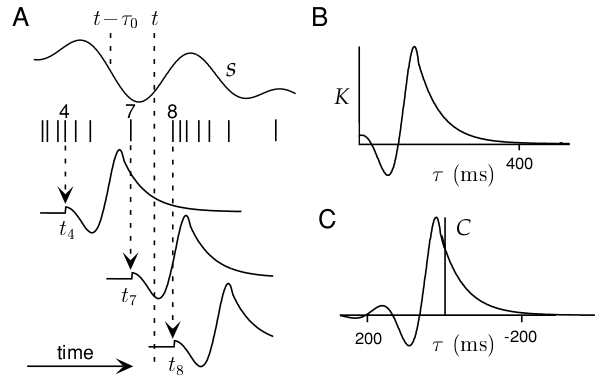
\includegraphics[scale = 0.4]{./png/3-13-A-B}
\end{center}
%\begin{center}
 %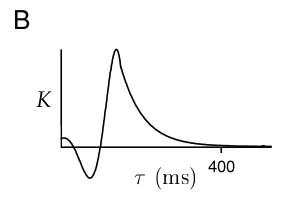
\includegraphics[scale = 0.5]{./png/3-13-B}

%\end{center}
\end{exm}


\begin{asm}
  \label{asm:ignore the causality}
  We ignore the causality constraint for now and construct
  an acausal kernel, but we will return to issues of causality later in the discussion.
\end{asm}

\begin{prop}
 Equation \ref{eq:3.51} can be written
in a compact way by using the neural response function
$\rho(t)\sum\delta(t-t_{i})$ introduced in chapter 1,
\begin{equation}
  \label{eq:3.52}
  s_{\rm{est}(t-\tau_{0})}=\int_{\infty}^{\infty}(\rho(t-\tau)-\left\langle r \right\rangle)K(\tau)d\tau.
\end{equation}
Using this form of the estimate, the construction of the optimal kernel $K$
proceeds very much like the construction of the optimal kernel for predicting firing rates in chapter 2.
\end{prop}

\begin{prop}
  We choose $K$ so that the squared difference
between the estimated stimulus and the actual stimulus, averaged over
both time and trials,
\begin{equation}
  \label{eq:3.53}
  \frac{1}{T}\int_0^T{\left\langle \left(
        \int_{-\infty}^{\infty}(\rho(t-\tau)-\left\langle r
        \right\rangle)K(\tau)-s(t-\tau_{0}) \right)^{2} \right\rangle d\tau},
\end{equation}
is minimized.
 \begin{proof}
  Using the calculus of variations,the result is that optimal kernal $K$ obeys the equation
\begin{equation}
  \label{eq:3.54}
  \int_{\infty}^{\infty}Q_{\rho\rho}(\tau-\tau')K(\tau')d\tau'=Q_{\rm{r}s}(\tau-\tau_{0}),
\end{equation}
where $Q_{\rho\rho}$ is the spike-train autocorrelation function,
\begin{equation}
  \label{eq:3.55}
  Q_{\rho\rho}=\frac{1}{T}\int_0^T{\left\langle
      (\rho(t-\tau)-\left\langle r
      \right\rangle)(\rho(t-\tau')-\left\langle r \right\rangle)
    \right\rangle dt},
\end{equation}
as defined in chapter 1. $Q_{\rm{r}s}$ is the correlation of the firing rate and the stimulus, which is related to the spike-triggered average $C$, both introduced in
chapter 1,
\begin{equation}
  \label{equ:3.56}
Q_{\rm{r}s}(\tau-\tau_{0})=\left\langle r \right\rangle C(\tau_0-\tau)=\frac{1}{T}\left\langle \sum\limits_{i=1}^{n}{s(t_i+\tau-\tau_{0})} \right\rangle,
\end{equation}
which completes the proof.
\end{proof}
\end{prop}

\begin{exm}
  If the spike train is uncorrelated, which tends to happen at low
  rates,
  \begin{equation}
    \label{eq:3.57}
    Q_{\rho\rho}=\left\langle r \right\rangle\delta(\tau),
  \end{equation}
  and we find from Equation \ref{eq:3.54} that
  \begin{equation}
    \label{eq:3.58}
    \begin{aligned}
          K(\tau)&=\frac{1}{\left\langle r
                   \right\rangle}Q_{\rm{r}s}(\tau-\tau_{0})=C(\tau_{0}-\tau)\\
      &=\frac{1}{\left\langle n \right\rangle}\left\langle \sum\limits_{i=1}^{n}{s(t_i+\tau-\tau_{0})} \right\rangle.
    \end{aligned}
  \end{equation}
  This is the average value of the stimulus at time $\tau-\tau_{0}$
  relative to the appearance of a spike. The figure C in Example \ref{exm:3_13ABC} is the
spike-triggered average corresponding to the kernel shown in figure B, assuming no spike-train correlations.
\end{exm}

\begin{rem}
   Because $\tau-\tau_{0}$ can be either positive or negative, stimulus
   estimation involves both forward and backward correlation and the
   average values of the stimulus both before and after a
   spike. Decoding in this way follows a simple rule: every time a
   spike appears, we replace it with the average stimulus surrounding a spike, shifted by an amount $\tau_{0}$.
\end{rem}

\begin{rem}
  Correlations between a spike and subsequent
stimuli can arise, in a causal system, only from correlations between the
stimulus and itself. If these are absent, as for white noise, $K(\tau)$ will be $0$
for $\tau>\tau_{0}$. For causal decoding, we must also have
$K(\tau)=0$ for $\tau<0$. Thus, if $\tau_0=0$ and the stimulus is uncorrelated, $K(\tau)=0$
for all values of $\tau$.
\end{rem}

\begin{prop}
When the spike-train autocorrelation function is not a $\delta$ function, an
acausal solution for $K$ can be expressed as an inverse Fourier transform,
\begin{equation}
  \label{eq:3.59}
  K(\tau)=\frac{1}{2\pi}\int{\tilde{K}(\omega)\exp(-i\omega\tau)},
\end{equation}
where
\begin{equation}
  \label{eq:3.60}
  \tilde{K}(\omega)=\frac{\tilde{Q}_{\rm{r}s}(\omega)\exp(-i\omega\tau_0)}{\tilde{Q}_{\rho\rho}(\omega)}.
\end{equation}
Here $\tilde{Q}_{\rm{r}s}$ and $\tilde{Q}_{\rho\rho}$ are the Fourier
transforms of ${Q}_{\rm{r}s}$ and ${Q}_{\rho\rho}$.
\end{prop}

\begin{exm}
  \label{exm:spike-train decoding for the H1 neuron}
  The figure shows an example of spike-train decoding for the H1 neuron
of the fly discussed in chapter 2. Flies have two H1 neurons, one on
each side of the body, that respond to motion in opposite
directions. As is often the case, half-wave rectification prevents a
single neuron from encoding both directions of motion. The top panel
gives two reconstruction kernels, one acausal and one causal. The two
rows of spikes in the middle panel shows typical responses of the H1
neuron to the stimuli (upper trace)  $s(t)$ and its negative,
$-s(t)$(bottom trace). This procedure provides a reasonable
approximation of recording both H1 neurons, and produces a
neuron/anti-neuron pair of recordings. The stimulus is then decoded by summing the kernel $K(t-t_{i})$ for all spike times $t_{i}$ of
the recorded H1 neuron and summing $-K(t-t_{i})$ for all spike times $t_{j}$ of its anti-neuron partner. The dashed line in the lower panel shows the actual stimulus, and the solid line
is the estimated stimulus from the optimal linear reconstruction using the acausal
filter.
\begin{center}
  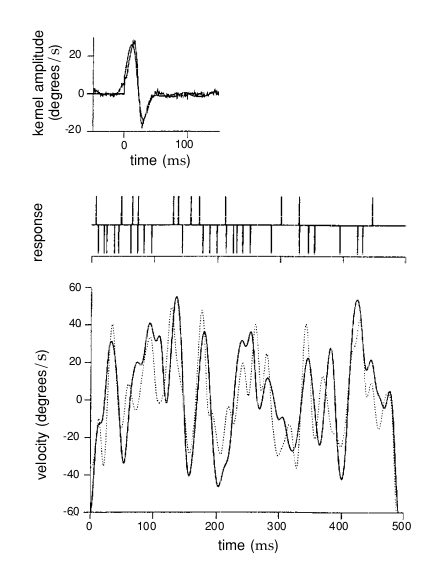
\includegraphics[scale = 0.5]{./png/3-14}
\end{center}
\end{exm}
%%% Local Variables:
%%% mode: latex
%%% TeX-master: "../notesOnFluidMechanics"
%%% End:
